The design approach is a JEE Architecture which is based on a client-server 4-tier distributed system.
\\Here we provide for each tier the definition, choice reasons and used technology:

\begin{itemize}
\item \textbf{Client Tier:} this tier is responsible of translating user actions and presenting the output of tasks and results into something the user can understand;

\item \textbf{Web Tier:} it receives the requests from the client tier and forwards the pieces of data collected to the business tier waiting for processed data to be sent to the client tier.
\\
Web Tier is composed by web beans. This tier purpose is the one to interact with the beans in the Business Logic tier and display data according to the user requests.

\item \textbf{Business Logic Tier:} this tier contains the business logic, it coordinates the application, processes commands, makes logical decisions and evaluations and performs computations.\\
It is responsible for the communication between the Web Tier and the Persistence Tier. Its components are the EJB Beans.


\item \textbf{Persistence Tier:} this tier holds the information of the system data model and is in charge of storing and retrieving information from the database.
\\
The persistence tier is composed of the entity beans which represent the entities depicted from our RASD document and then further endorsed in our conceptual design. These entities are fundamental as they represent the connection to our database. Since in JEE we are interested in working in an object oriented environment, they represent a high level object view of the database.\\
In particular, for Travlendar+ it will be used a relational DBMS: MySQL, and the JPA standards of JEE in order to look and use the database entities in a object oriented way.
\end{itemize}

\begin{figure}[ph]
\centering
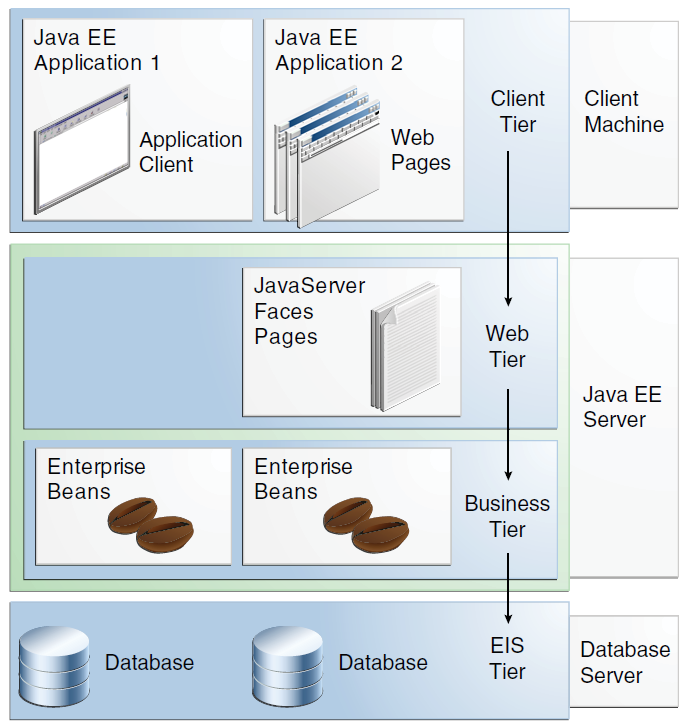
\includegraphics[width=\linewidth]{./images/jeearch}
\caption[jee arch]{JEE architecture}
\label{fig:jeearch}
\end{figure}